\section{Техническое задание}
\subsection{Основание для разработки}

Основанием для разработки является задание на выпускную квалификационную работу по теме «Проектирование и разработка онлайн-платформы с базой данных для поиска работы и подбора IT-специалистов».

Разработка программной системы выполняется в рамках выпускной квалификационной работы по направлению 09.03.04 «Программная инженерия».

\subsection{Цель и назначение разработки}

Целью разработки является проектирование и разработка онлайн-платформы с базой данных для поиска работы и подбора IT-специалистов.

Назначение разрабатываемой программной системы заключается в обеспечении взаимодействия между соискателями, работодателями и администратором в рамках процессов размещения вакансий, поиска кандидатов, отправки откликов и контроля этапов их обработки.

Программная система предназначена для хранения и обработки данных о пользователях, профилях соискателей, компаниях, вакансиях, откликах, избранных вакансиях и навыках, а также для поддержки основных операций, связанных с поиском работы и подбором IT-специалистов.

\subsection{Задачи разработки}

На основании проведённого анализа предметной области поиска работы и подбора IT-специалистов формулируются основные задачи разработки:
\begin{enumerate}
	\item Провести анализ предметной области поиска работы и подбора IT-специалистов, выявить основные требования к разрабатываемой платформе и сформировать техническое задание.
	\item Спроектировать архитектуру программной системы и структуру данных, обеспечивающие хранение и обработку сведений о пользователях, профилях соискателей, компаниях, вакансиях, навыках, откликах и избранных вакансиях.
	\item Спроектировать базу данных и пользовательский интерфейс программной системы с учётом ролей соискателя, работодателя, администратора и неавторизованного пользователя.
	\item Реализовать программную систему, обеспечивающую выполнение основных функций, связанных с регистрацией и авторизацией пользователей, ведением профилей и компаний, размещением вакансий, поиском информации, обработкой откликов и выполнением административных действий.
	\item Провести тестирование основных сценариев взаимодействия пользователей с платформой и оформить программную документацию.
\end{enumerate}

Сформулированные задачи отражают основные этапы разработки программной системы и определяют направления её последующего проектирования и реализации.

\subsection{Требования к программной системе}

\subsubsection{Требования к данным программной системы}

В программной системе должны храниться и обрабатываться следующие данные:
\begin{itemize}
	\item данные пользователей, включая адрес электронной почты, хэш пароля, роль пользователя, имя и фамилию, а также признак блокировки;
	\item данные профиля соискателя, включая специализацию, краткую информацию о пользователе и ссылку на GitHub-профиль;
	\item данные компании работодателя, включая название компании, описание и адрес web-сайта;
	\item данные вакансий, включая название, специализацию, описание, требования к кандидату, заработную плату, местоположение, тип занятости, формат работы, статус вакансии и дату создания;
	\item данные откликов, включая связь между вакансией и профилем соискателя, статус отклика и дату его отправки;
	\item данные об избранных вакансиях, сохраняемых пользователем;
	\item данные о навыках, используемых в системе;
	\item данные о навыках соискателя;
	\item данные о навыках, требуемых для вакансии.
\end{itemize}

Роли соискателя, работодателя/рекрутера и администратора не выделяются в отдельные сущности и задаются как значение роли пользователя. Работодатель и рекрутер рассматриваются в системе как одна роль. Отдельная сущность резюме не создаётся, её функцию выполняет профиль соискателя. Отдельные сущности профиля работодателя, чата, жалоб и избранных кандидатов в системе не предусматриваются.

Между данными программной системы должны поддерживаться следующие основные связи и ограничения:
\begin{itemize}
	\item одному пользователю с ролью соискателя может соответствовать один профиль соискателя;
	\item одному пользователю с ролью работодателя может соответствовать одна компания;
	\item одна компания может быть связана с несколькими вакансиями;
	\item один профиль соискателя может быть связан с несколькими откликами;
	\item одна вакансия может быть связана с несколькими откликами;
	\item один и тот же профиль соискателя не может отправить более одного отклика на одну и ту же вакансию;
	\item один и тот же пользователь не может сохранить одну и ту же вакансию в избранное более одного раза;
	\item навыки соискателя и навыки вакансии должны храниться через отдельные сущности связи;
	\item статусы вакансии должны поддерживать состояния draft, published и archived;
	\item статусы отклика должны поддерживать состояния new, in\_review, accepted и rejected.
\end{itemize}

\subsubsection{Функциональные требования к программной системе}

Программная система должна обеспечивать выполнение функций, связанных с регистрацией и авторизацией пользователей, ведением профилей, размещением вакансий, обработкой откликов, поиском информации и базовыми административными действиями.

Для соискателя в системе должны быть предусмотрены следующие функции:
\begin{itemize}
	\item регистрация в системе;
	\item вход в систему и выход из неё;
	\item создание и редактирование профиля соискателя;
	\item добавление и удаление навыков профиля;
	\item просмотр списка опубликованных вакансий;
	\item поиск и фильтрация вакансий;
	\item просмотр карточки вакансии;
	\item отправка отклика на вакансию;
	\item просмотр своих откликов;
	\item добавление вакансии в избранное;
	\item удаление вакансии из избранного;
	\item просмотр списка избранных вакансий.
\end{itemize}

Для работодателя в системе должны быть предусмотрены следующие функции:
\begin{itemize}
	\item регистрация в системе;
	\item вход в систему и выход из неё;
	\item создание и редактирование данных компании;
	\item создание вакансий;
	\item редактирование вакансий;
	\item публикация вакансий;
	\item снятие вакансий с публикации;
	\item добавление и удаление навыков вакансии;
	\item просмотр списка своих вакансий;
	\item просмотр откликов на вакансии;
	\item изменение статусов откликов;
	\item поиск и фильтрация профилей соискателей.
\end{itemize}

Для администратора в системе должны быть предусмотрены следующие функции:
\begin{itemize}
	\item вход в систему и выход из неё;
	\item просмотр списка пользователей;
	\item просмотр списка вакансий;
	\item блокировка пользователей;
	\item снятие вакансий с публикации;
	\item удаление вакансий.
\end{itemize}

Программная система должна обеспечивать разграничение функциональных возможностей в зависимости от роли пользователя и не допускать выполнения действий, не предусмотренных для соответствующей роли.

\subsubsection{Требования к интерфейсу}

Интерфейс программной системы должен быть реализован в виде web-интерфейса и обеспечивать удобный доступ к основным функциям системы в зависимости от роли пользователя.

Интерфейс должен включать страницы и формы, необходимые для выполнения операций регистрации, авторизации, работы с профилем соискателя, работы с компанией, размещения вакансий, отправки и обработки откликов, просмотра избранных вакансий и выполнения административных действий.

Для неавторизованного пользователя должен быть обеспечен доступ к просмотру списка опубликованных вакансий, фильтрации вакансий, просмотру карточки вакансии, а также к страницам входа и регистрации. Внешний вид страницы списка вакансий представлен на рисунке~\ref{fig:vacancies-list}.

\begin{figure}[H]
	\centering
	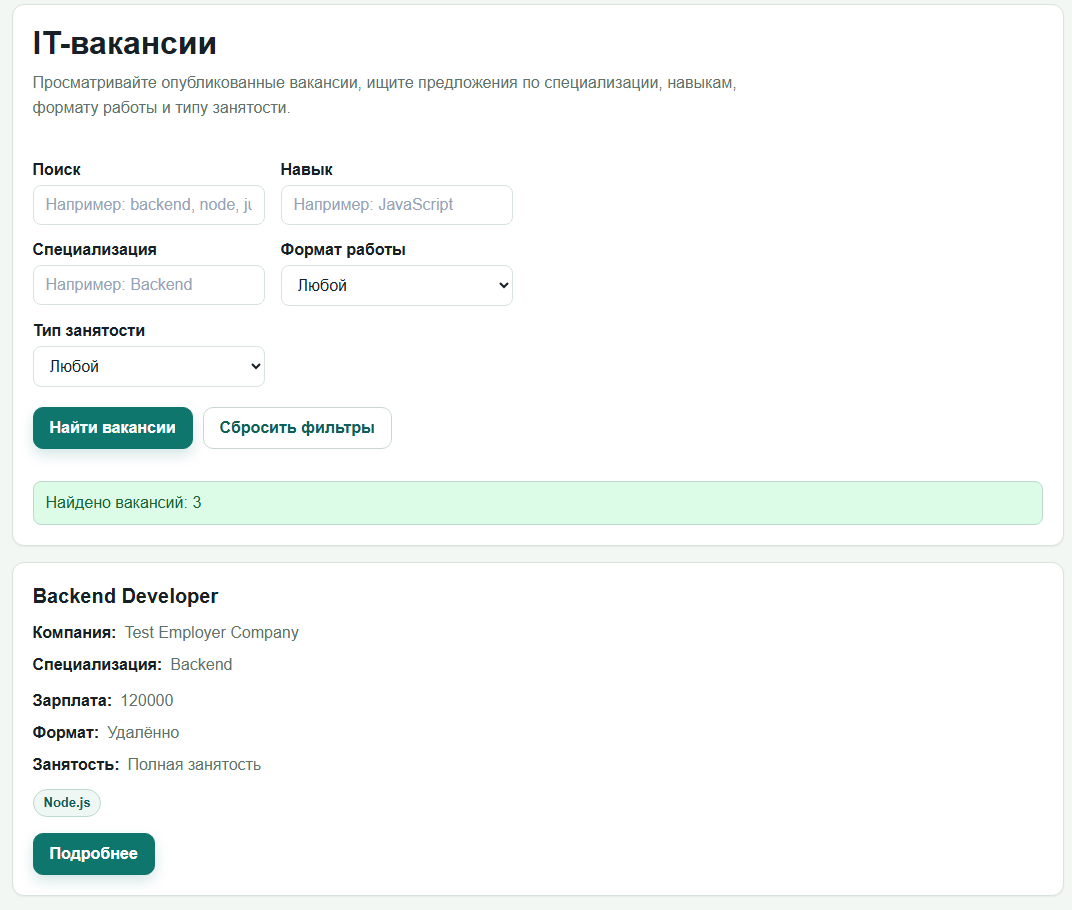
\includegraphics[width=\linewidth]{vacancies_list}
	\caption{Страница списка вакансий}
	\label{fig:vacancies-list}
\end{figure}

Как показано на рисунке~\ref{fig:vacancies-list}, страница списка вакансий содержит заголовок раздела, блок фильтрации, сведения о количестве найденных вакансий и список доступных предложений.

Для соискателя интерфейс должен обеспечивать доступ к просмотру и редактированию профиля, управлению навыками, просмотру вакансий, просмотру карточки вакансии, отправке откликов, просмотру своих откликов, а также к просмотру и управлению избранными вакансиями. Внешний вид страницы карточки вакансии представлен на рисунке~\ref{fig:vacancy-card}.

\begin{figure}[H]
	\centering
	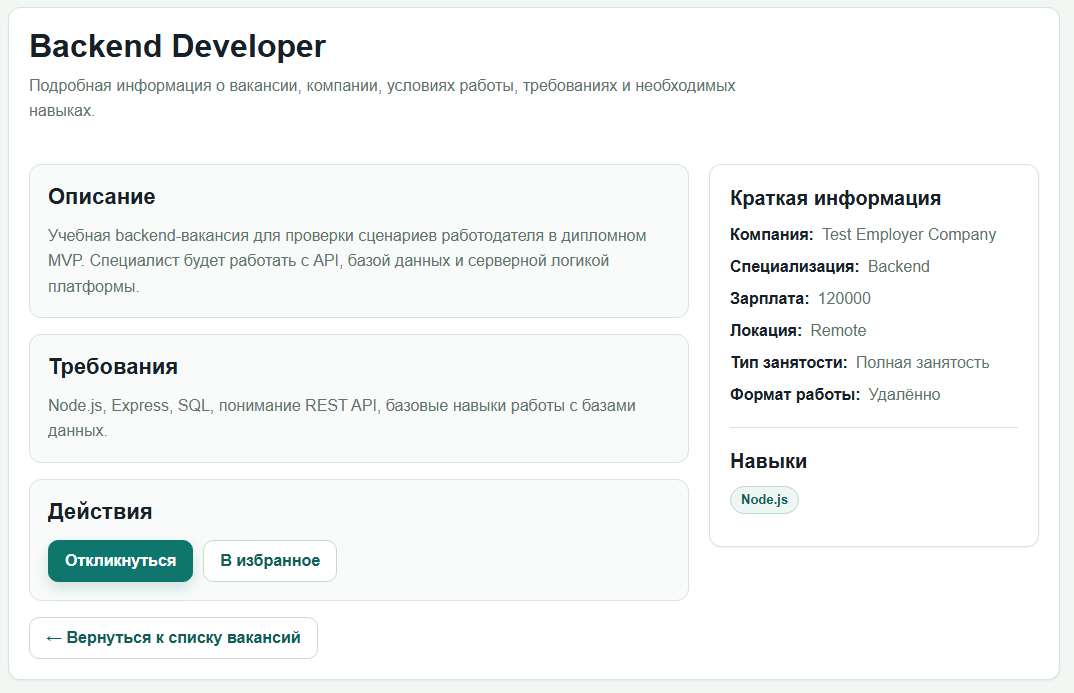
\includegraphics[width=\linewidth]{vacancy_card}
	\caption{Страница карточки вакансии}
	\label{fig:vacancy-card}
\end{figure}

Как показано на рисунке~\ref{fig:vacancy-card}, страница карточки вакансии содержит подробную информацию о выбранной вакансии, требованиях к кандидату, навыках и доступных действиях со стороны пользователя.

Для работодателя интерфейс должен обеспечивать доступ к просмотру и редактированию данных компании, созданию и редактированию вакансий, управлению публикацией вакансий, управлению навыками вакансии, просмотру откликов и фильтрации профилей соискателей. Внешний вид страницы работодателя со списком вакансий представлен на рисунке~\ref{fig:employer-vacancies}.

\begin{figure}[H]
	\centering
	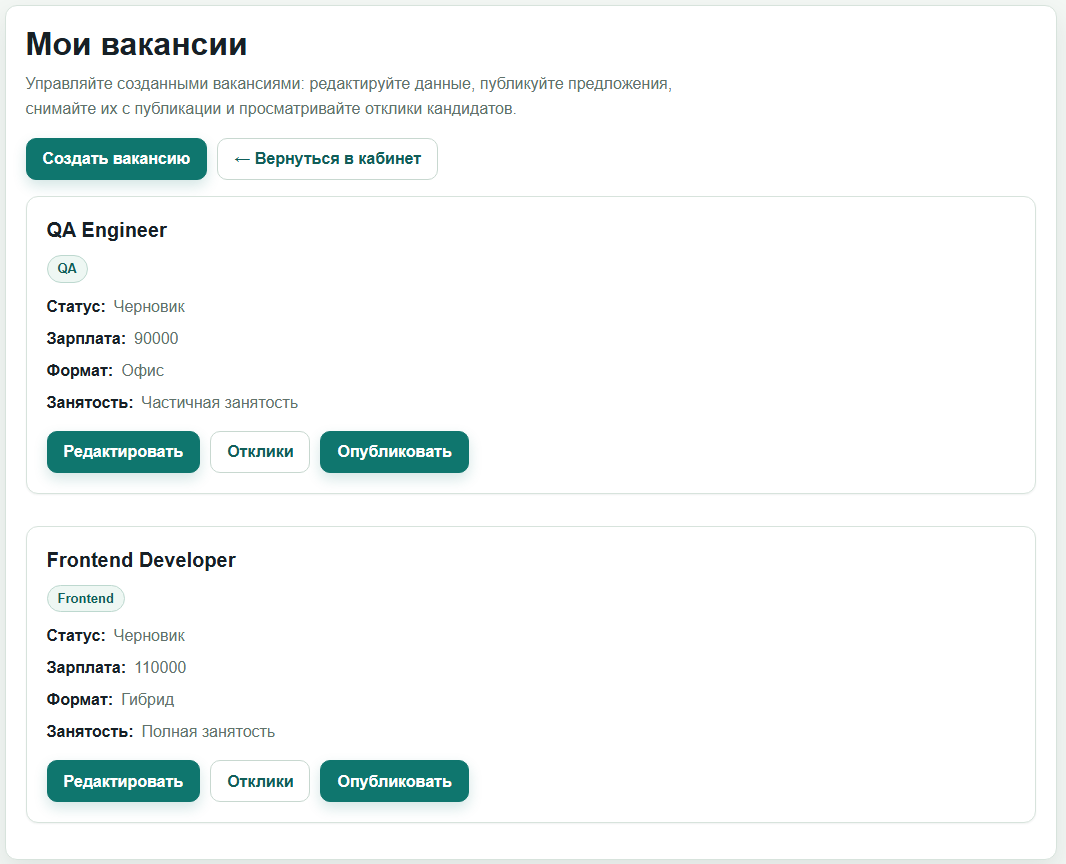
\includegraphics[width=\linewidth]{employer_vacancies}
	\caption{Страница работодателя со списком вакансий}
	\label{fig:employer-vacancies}
\end{figure}

Как показано на рисунке~\ref{fig:employer-vacancies}, страница работодателя содержит список созданных вакансий, сведения об их параметрах и элементы управления, связанные с редактированием, публикацией и просмотром откликов.

Для администратора интерфейс должен обеспечивать доступ к просмотру пользователей, просмотру вакансий, блокировке пользователей, снятию вакансий с публикации и удалению вакансий.

Интерфейс программной системы должен обеспечивать логичную навигацию между страницами, отображение результатов пользовательских действий, отображение сообщений об ошибках при некорректном вводе данных или попытке выполнения недопустимых действий, а также разграничение доступных элементов интерфейса в зависимости от роли пользователя.

\subsubsection{Требования к надёжности}

Программная система должна обеспечивать корректную обработку пользовательских действий и сохранение целостности данных при выполнении основных операций.

При вводе некорректных, неполных или недопустимых данных система должна предотвращать выполнение ошибочных операций и выводить пользователю сообщение об ошибке.

Система должна обеспечивать сохранение согласованности данных при работе с пользователями, профилями соискателей, компаниями, вакансиями, откликами, избранными вакансиями и навыками.

Система не должна допускать выполнение действий, нарушающих установленные ограничения предметной области, включая повторную отправку отклика на одну и ту же вакансию одним и тем же профилем соискателя, повторное добавление одной и той же вакансии в избранное одним и тем же пользователем, а также выполнение действий, не соответствующих роли пользователя.

При выполнении операций изменения данных система должна обеспечивать корректную обработку статусов вакансий и откликов, а также сохранение связей между сущностями программной системы.

В случае возникновения ошибок при обработке запроса система должна завершать операцию без нарушения целостности хранимых данных.

\subsubsection{Требования к информационной безопасности}

Программная система должна обеспечивать защиту данных пользователей и разграничение доступа к функциям и данным в зависимости от роли пользователя.

Доступ к функциям, связанным с изменением данных, должен предоставляться только авторизованным пользователям. Аутентификация пользователей должна выполняться на основе пары электронная почта и пароль.

Пароли пользователей не должны храниться в открытом виде и должны сохраняться в системе в виде хэша.

Авторизация пользователей в программной системе должна осуществляться с использованием JWT-токенов.

Программная система должна обеспечивать разграничение прав доступа между соискателем, работодателем и администратором. Пользователь не должен иметь возможность выполнять действия и получать доступ к данным, не предусмотренным его ролью.

Система должна ограничивать доступ пользователя к изменению только тех данных, которые относятся к его собственной учётной записи, профилю, компании, вакансиям, откликам и иным связанным объектам в пределах предоставленных прав.

Для пользователей, имеющих признак блокировки, должен быть запрещён доступ к использованию функциональных возможностей системы.

\subsubsection{Требования к программной и технической совместимости}

Программная система должна функционировать как web-приложение, доступ к которому осуществляется через web-интерфейс.

Серверная часть программной системы должна быть реализована с использованием Node.js и Express. Клиентская часть должна быть реализована на HTML, CSS и JavaScript без использования отдельного frontend-приложения.

Для хранения данных в системе должна использоваться система управления базами данных PostgreSQL.

Программная система должна поддерживать работу в монолитной клиент-серверной архитектуре, в которой серверное приложение одновременно обеспечивает обработку запросов, бизнес-логику и выдачу страниц пользовательского интерфейса.

Для развёртывания и запуска программной системы должно использоваться контейнерное окружение Docker.

Программная система предназначена для использования на персональном компьютере и не предполагает отдельной мобильной версии или мобильного приложения.

\subsection{Варианты использования программы}

Для разрабатываемой программной системы выделяются следующие акторы: гость, соискатель, работодатель и администратор.

Диаграммы прецедентов, отражающие взаимодействие указанных акторов с программной системой, представлены на рисунках~\ref{fig:guest-usecase}--\ref{fig:admin-usecase}.

На диаграммах представлены основные действия пользователей, связанные с просмотром вакансий, работой с профилем соискателя, размещением вакансий, обработкой откликов и выполнением административных функций.

\begin{figure}[H]
	\centering
	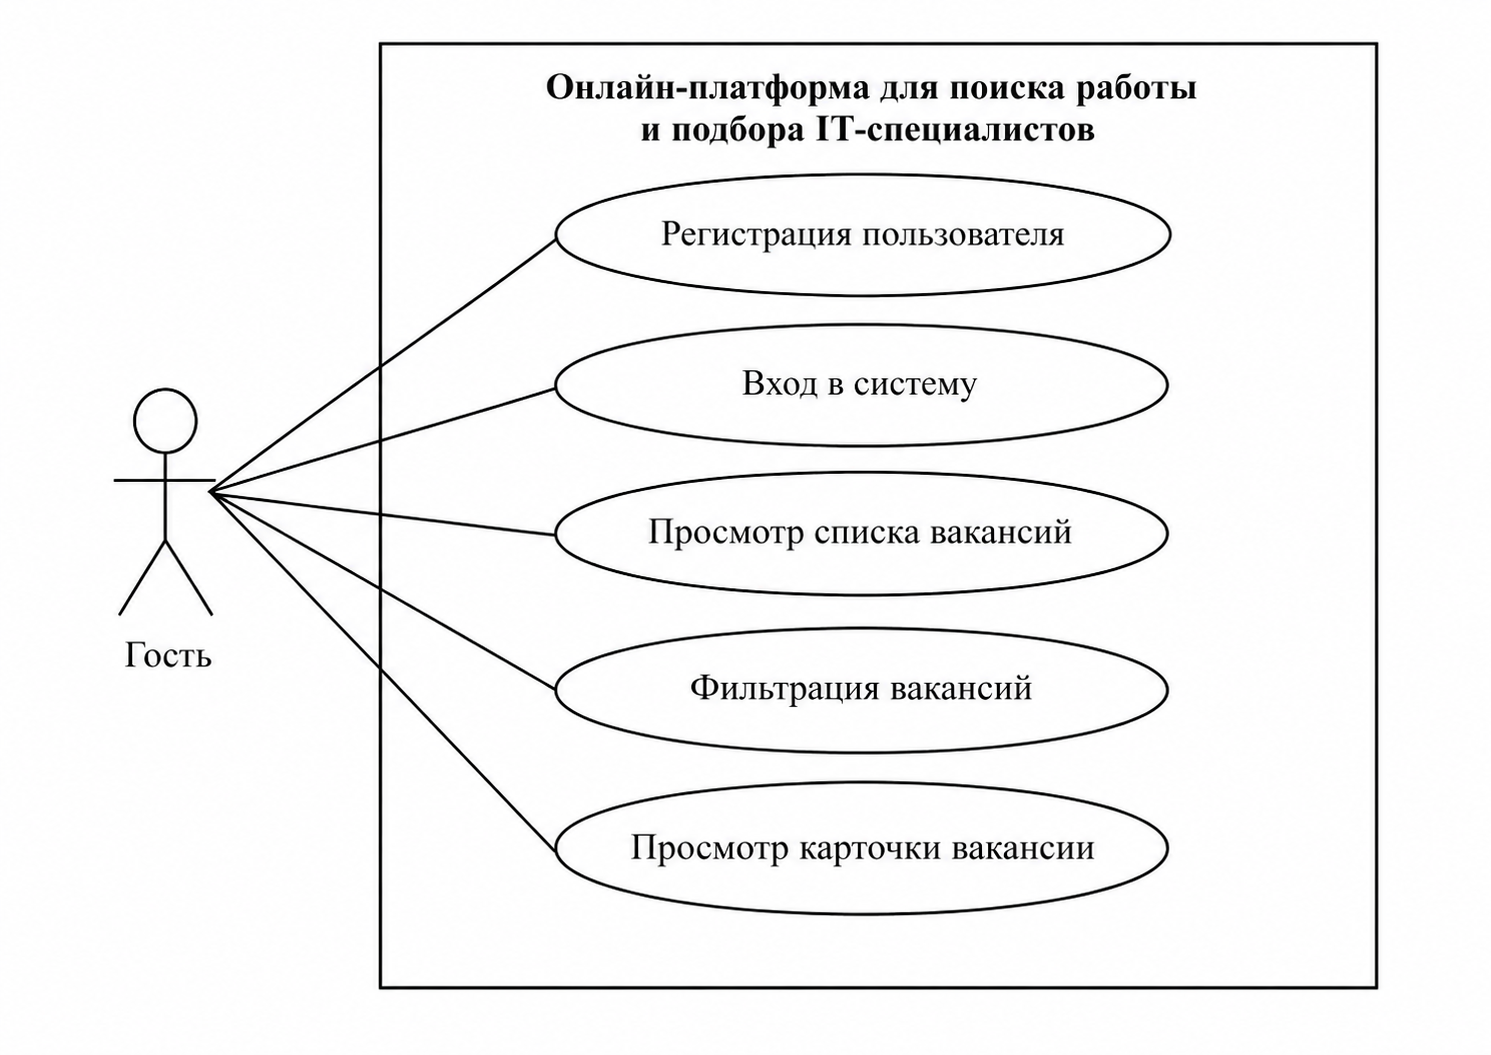
\includegraphics[width=0.88\linewidth]{guest_usecase}
	\caption{Диаграмма прецедентов для актора «Гость»}
	\label{fig:guest-usecase}
\end{figure}

\begin{figure}[H]
	\centering
	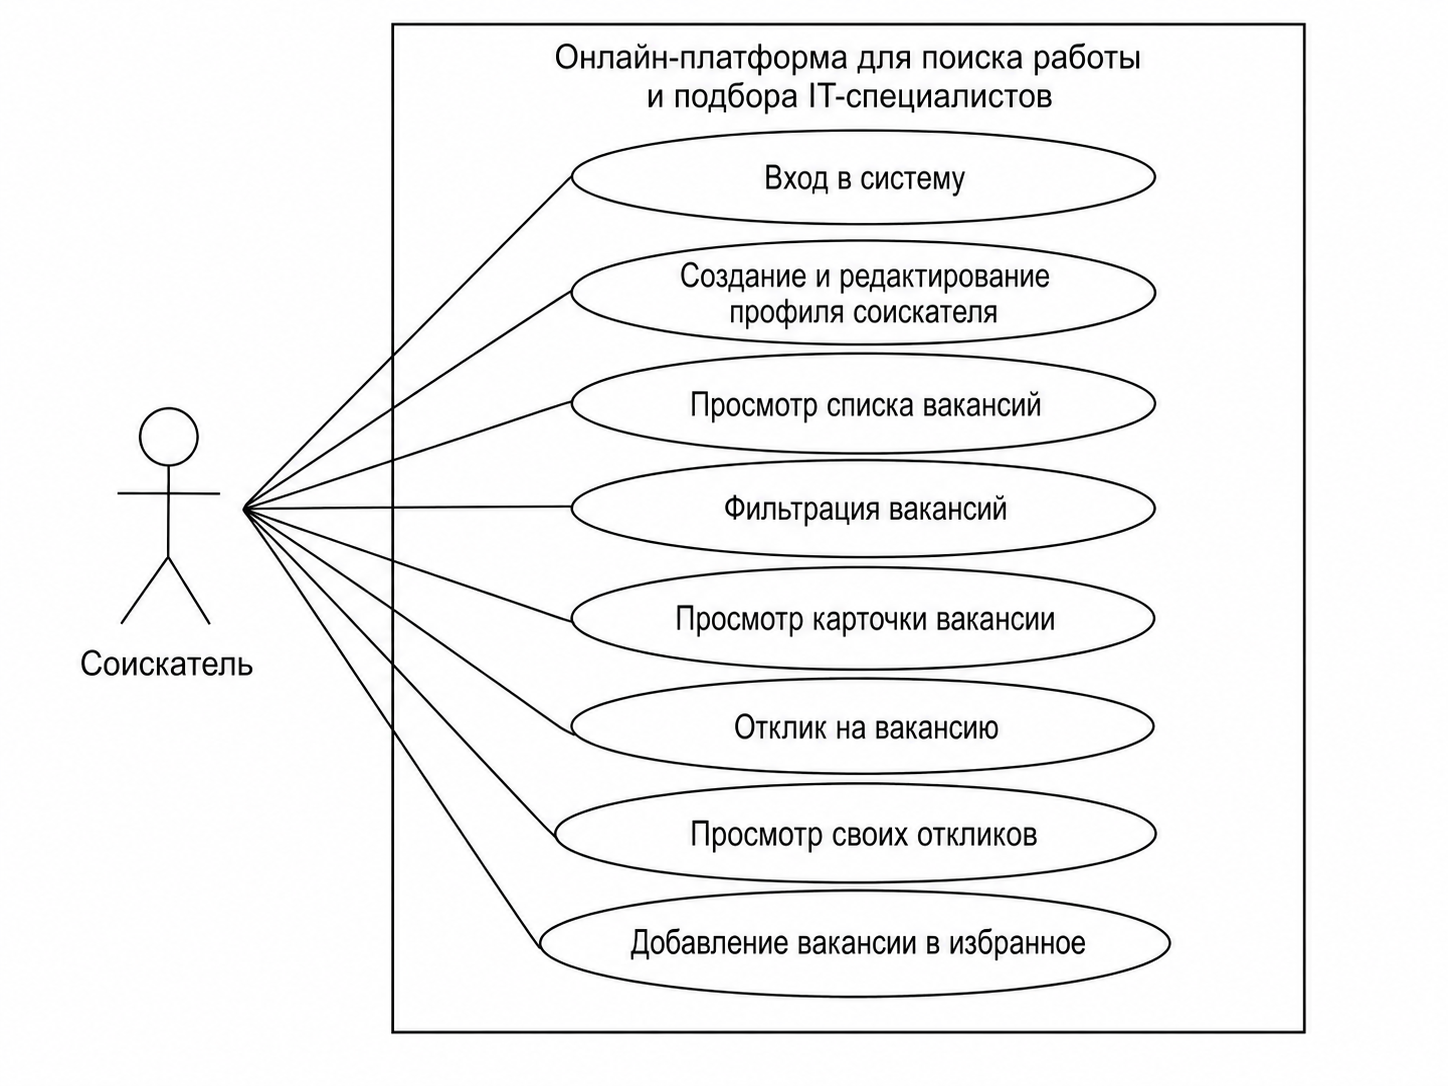
\includegraphics[width=0.88\linewidth]{jobseeker_usecase}
	\caption{Диаграмма прецедентов для актора «Соискатель»}
	\label{fig:jobseeker-usecase}
\end{figure}

\begin{figure}[H]
	\centering
	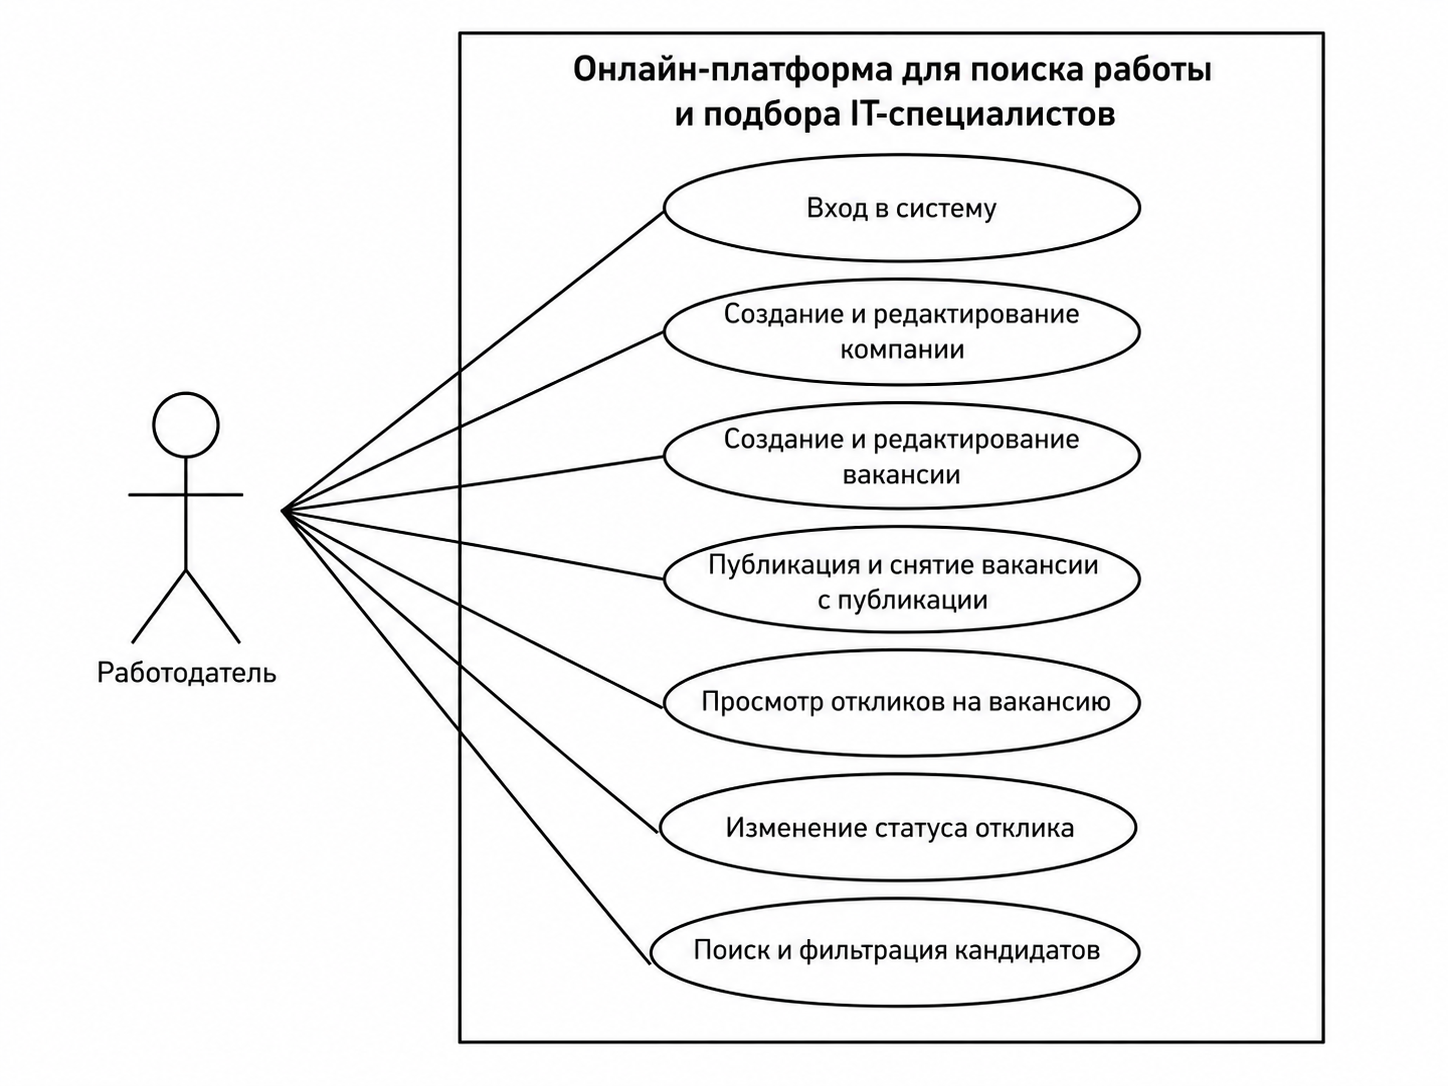
\includegraphics[width=0.88\linewidth]{employer_usecase}
	\caption{Диаграмма прецедентов для актора «Работодатель»}
	\label{fig:employer-usecase}
\end{figure}

\begin{figure}[H]
	\centering
	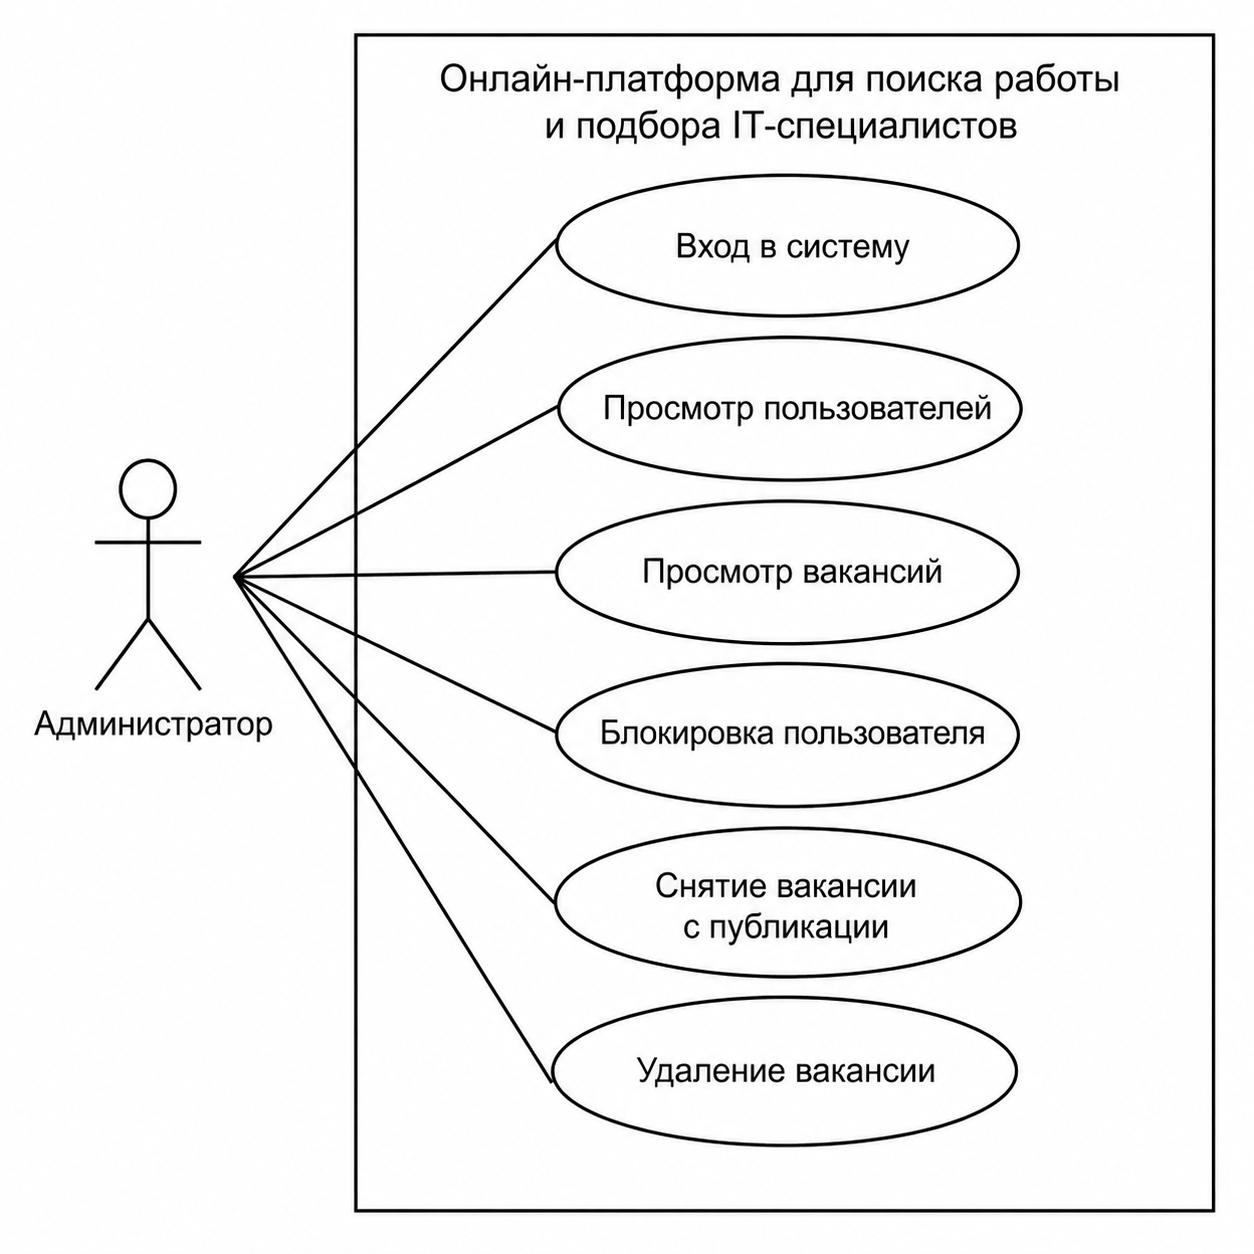
\includegraphics[width=0.77\linewidth]{admin_usecase}
	\caption{Диаграмма прецедентов для актора «Администратор»}
	\label{fig:admin-usecase}
\end{figure}

\subsubsection{Вариант использования «Регистрация пользователя»}

\textbf{Заинтересованное лицо:} неавторизованный пользователь.

\textbf{Предусловие:} пользователь открыл страницу регистрации в программной системе.

\textbf{Постусловие:} в системе создана новая учетная запись пользователя с ролью соискателя или работодателя.

\textbf{Основной сценарий:}
\begin{enumerate}
	\item Пользователь переходит на страницу регистрации.
	\item Пользователь вводит регистрационные данные.
	\item Пользователь выбирает роль соискателя или работодателя.
	\item Система выполняет проверку корректности введенных данных.
	\item Система создает новую учетную запись пользователя.
	\item Система сохраняет данные пользователя в базе данных.
\end{enumerate}

\textbf{Альтернативный сценарий:}
\begin{enumerate}
	\item Пользователь вводит некорректные, неполные или уже использованные регистрационные данные.
	\item Система не выполняет регистрацию пользователя.
	\item Система выводит сообщение об ошибке.
\end{enumerate}

\subsubsection{Вариант использования «Вход в систему»}

\textbf{Заинтересованное лицо:} пользователь.

\textbf{Предусловие:} пользователь имеет учетную запись в программной системе и открыл страницу входа.

\textbf{Постусловие:} пользователь авторизован в системе и получает доступ к функциям, предусмотренным его ролью.

\textbf{Основной сценарий:}
\begin{enumerate}
	\item Пользователь переходит на страницу входа.
	\item Пользователь вводит адрес электронной почты и пароль.
	\item Пользователь отправляет форму входа.
	\item Система проверяет корректность введенных учетных данных.
	\item Система выполняет авторизацию пользователя.
	\item Пользователь получает доступ к функциям системы в соответствии со своей ролью.
\end{enumerate}

\textbf{Альтернативный сценарий:}
\begin{enumerate}
	\item Пользователь вводит неверные учетные данные или оставляет обязательные поля незаполненными.
	\item Система не выполняет авторизацию пользователя.
	\item Система выводит сообщение об ошибке.
\end{enumerate}

\subsubsection{Вариант использования «Создание и редактирование профиля соискателя»}

\textbf{Заинтересованное лицо:} соискатель.

\textbf{Предусловие:} пользователь авторизован в системе с ролью соискателя.

\textbf{Постусловие:} профиль соискателя создан или обновлен.

\textbf{Основной сценарий:}
\begin{enumerate}
	\item Соискатель переходит к странице профиля.
	\item Соискатель вводит или изменяет данные профиля.
	\item Соискатель сохраняет внесенные изменения.
	\item Система проверяет корректность введенных данных.
	\item Система создает профиль соискателя или обновляет ранее сохраненные данные.
	\item Система сохраняет изменения в базе данных.
\end{enumerate}

\textbf{Альтернативный сценарий:}
\begin{enumerate}
	\item Соискатель вводит некорректные или неполные данные.
	\item Система не сохраняет изменения профиля.
	\item Система выводит сообщение об ошибке.
\end{enumerate}

\subsubsection{Вариант использования «Просмотр списка вакансий»}

\textbf{Заинтересованное лицо:} пользователь.

\textbf{Предусловие:} пользователь открыл страницу со списком вакансий.

\textbf{Постусловие:} пользователю отображен список опубликованных вакансий.

\textbf{Основной сценарий:}
\begin{enumerate}
	\item Пользователь переходит к странице со списком вакансий.
	\item Система получает данные об опубликованных вакансиях.
	\item Система формирует список вакансий.
	\item Система отображает пользователю список опубликованных вакансий.
\end{enumerate}

\textbf{Альтернативный сценарий:}
\begin{enumerate}
	\item В системе отсутствуют опубликованные вакансии.
	\item Система отображает пользователю сообщение об отсутствии доступных вакансий.
\end{enumerate}


\subsubsection{Вариант использования «Поиск и фильтрация вакансий»}

\textbf{Заинтересованное лицо:} пользователь.

\textbf{Предусловие:} пользователь открыл страницу со списком вакансий.

\textbf{Постусловие:} пользователю отображен список вакансий, соответствующих заданным параметрам фильтрации.

\textbf{Основной сценарий:}
\begin{enumerate}
	\item Пользователь переходит к странице со списком вакансий.
	\item Пользователь задает параметры фильтрации вакансий.
	\item Пользователь применяет выбранные параметры.
	\item Система получает параметры фильтрации.
	\item Система выполняет отбор вакансий, соответствующих заданным условиям.
	\item Система отображает пользователю обновленный список вакансий.
\end{enumerate}

\textbf{Альтернативный сценарий:}
\begin{enumerate}
	\item По заданным параметрам не найдено ни одной вакансии.
	\item Система отображает пользователю сообщение об отсутствии подходящих вакансий.
\end{enumerate}

\subsubsection{Вариант использования «Просмотр карточки вакансии»}

\textbf{Заинтересованное лицо:} пользователь.

\textbf{Предусловие:} пользователь открыл список вакансий или перешел по ссылке на конкретную вакансию.

\textbf{Постусловие:} пользователю отображена подробная информация о выбранной вакансии.

\textbf{Основной сценарий:}
\begin{enumerate}
	\item Пользователь выбирает вакансию из списка или переходит по ссылке на нее.
	\item Система получает данные о выбранной вакансии.
	\item Система формирует карточку вакансии.
	\item Система отображает пользователю подробную информацию о вакансии.
\end{enumerate}

\textbf{Альтернативный сценарий:}
\begin{enumerate}
	\item Выбранная вакансия отсутствует или недоступна для просмотра.
	\item Система не отображает карточку вакансии.
	\item Система выводит сообщение об ошибке.
\end{enumerate}

\subsubsection{Вариант использования «Отклик на вакансию»}

\textbf{Заинтересованное лицо:} соискатель.

\textbf{Предусловие:} пользователь авторизован в системе с ролью соискателя, имеет профиль соискателя и открыл карточку вакансии.

\textbf{Постусловие:} в системе создан новый отклик на выбранную вакансию.

\textbf{Основной сценарий:}
\begin{enumerate}
	\item Соискатель открывает карточку вакансии.
	\item Соискатель инициирует отправку отклика на вакансию.
	\item Система проверяет возможность создания отклика.
	\item Система создает новый отклик, связывающий профиль соискателя и выбранную вакансию.
	\item Система сохраняет отклик в базе данных.
	\item Система отображает результат успешной отправки отклика.
\end{enumerate}

\textbf{Альтернативный сценарий:}
\begin{enumerate}
	\item Соискатель уже отправлял отклик на выбранную вакансию либо выполнение операции невозможно.
	\item Система не создает новый отклик.
	\item Система выводит сообщение об ошибке.
\end{enumerate}

\subsubsection{Вариант использования «Просмотр своих откликов»}

\textbf{Заинтересованное лицо:} соискатель.

\textbf{Предусловие:} пользователь авторизован в системе с ролью соискателя.

\textbf{Постусловие:} соискателю отображен список ранее отправленных откликов с информацией об их статусах.

\textbf{Основной сценарий:}
\begin{enumerate}
	\item Соискатель переходит к разделу просмотра своих откликов.
	\item Система получает данные об откликах, связанных с профилем соискателя.
	\item Система формирует список откликов.
	\item Система отображает соискателю список его откликов и текущие статусы их обработки.
\end{enumerate}

\textbf{Альтернативный сценарий:}
\begin{enumerate}
	\item У соискателя отсутствуют ранее отправленные отклики.
	\item Система отображает сообщение об отсутствии откликов.
\end{enumerate}

\subsubsection{Вариант использования «Добавление вакансии в избранное»}

\textbf{Заинтересованное лицо:} соискатель.

\textbf{Предусловие:} пользователь авторизован в системе с ролью соискателя и открыл список вакансий или карточку вакансии.

\textbf{Постусловие:} выбранная вакансия добавлена в список избранных вакансий пользователя.

\textbf{Основной сценарий:}
\begin{enumerate}
	\item Соискатель открывает список вакансий или карточку вакансии.
	\item Соискатель инициирует добавление вакансии в избранное.
	\item Система проверяет возможность выполнения операции.
	\item Система добавляет выбранную вакансию в список избранных вакансий пользователя.
	\item Система сохраняет изменения в базе данных.
	\item Система отображает результат успешного выполнения операции.
\end{enumerate}

\textbf{Альтернативный сценарий:}
\begin{enumerate}
	\item Вакансия уже была ранее добавлена в избранное либо выполнение операции невозможно.
	\item Система не добавляет вакансию повторно.
	\item Система выводит сообщение об ошибке.
\end{enumerate}

\subsubsection{Вариант использования «Создание и редактирование компании»}

\textbf{Заинтересованное лицо:} работодатель.

\textbf{Предусловие:} пользователь авторизован в системе с ролью работодателя.

\textbf{Постусловие:} данные компании созданы или обновлены.

\textbf{Основной сценарий:}
\begin{enumerate}
	\item Работодатель переходит к разделу работы с данными компании.
	\item Работодатель вводит или изменяет данные компании.
	\item Работодатель сохраняет внесенные изменения.
	\item Система проверяет корректность введенных данных.
	\item Система создает данные компании или обновляет ранее сохраненные данные.
	\item Система сохраняет изменения в базе данных.
\end{enumerate}

\textbf{Альтернативный сценарий:}
\begin{enumerate}
	\item Работодатель вводит некорректные или неполные данные.
	\item Система не сохраняет изменения.
	\item Система выводит сообщение об ошибке.
\end{enumerate}

\subsubsection{Вариант использования «Создание и редактирование вакансии»}

\textbf{Заинтересованное лицо:} работодатель.

\textbf{Предусловие:} пользователь авторизован в системе с ролью работодателя и имеет созданные данные компании.

\textbf{Постусловие:} вакансия создана или обновлена.

\textbf{Основной сценарий:}
\begin{enumerate}
	\item Работодатель переходит к разделу работы с вакансиями.
	\item Работодатель инициирует создание новой вакансии или выбирает ранее созданную вакансию для редактирования.
	\item Работодатель вводит или изменяет данные вакансии.
	\item Работодатель сохраняет внесенные изменения.
	\item Система проверяет корректность введенных данных.
	\item Система создает новую вакансию или обновляет ранее сохраненные данные вакансии.
	\item Система сохраняет изменения в базе данных.
\end{enumerate}

\textbf{Альтернативный сценарий:}
\begin{enumerate}
	\item Работодатель вводит некорректные или неполные данные вакансии.
	\item Система не сохраняет изменения.
	\item Система выводит сообщение об ошибке.
\end{enumerate}

\subsubsection{Вариант использования «Публикация и снятие вакансии с публикации»}

\textbf{Заинтересованное лицо:} работодатель.

\textbf{Предусловие:} пользователь авторизован в системе с ролью работодателя и имеет ранее созданную вакансию.

\textbf{Постусловие:} статус вакансии изменен, в результате чего вакансия становится опубликованной или снимается с публикации.

\textbf{Основной сценарий:}
\begin{enumerate}
	\item Работодатель переходит к списку своих вакансий.
	\item Работодатель выбирает вакансию, для которой необходимо изменить статус публикации.
	\item Работодатель инициирует публикацию вакансии или снятие ее с публикации.
	\item Система проверяет возможность выполнения операции.
	\item Система изменяет статус вакансии.
	\item Система сохраняет изменения в базе данных.
	\item Система отображает результат успешного выполнения операции.
\end{enumerate}

\textbf{Альтернативный сценарий:}
\begin{enumerate}
	\item Выполнение операции публикации или снятия вакансии с публикации невозможно.
	\item Система не изменяет статус вакансии.
	\item Система выводит сообщение об ошибке.
\end{enumerate}

\subsubsection{Вариант использования «Просмотр откликов на вакансию»}

\textbf{Заинтересованное лицо:} работодатель.

\textbf{Предусловие:} пользователь авторизован в системе с ролью работодателя и открыл раздел просмотра откликов по выбранной вакансии.

\textbf{Постусловие:} работодателю отображен список откликов, связанных с выбранной вакансией.

\textbf{Основной сценарий:}
\begin{enumerate}
	\item Работодатель переходит к списку своих вакансий.
	\item Работодатель выбирает вакансию, для которой необходимо просмотреть отклики.
	\item Система получает данные об откликах, связанных с выбранной вакансией.
	\item Система формирует список откликов.
	\item Система отображает работодателю список откликов по выбранной вакансии.
\end{enumerate}

\textbf{Альтернативный сценарий:}
\begin{enumerate}
	\item Для выбранной вакансии отсутствуют отклики.
	\item Система отображает сообщение об отсутствии откликов.
\end{enumerate}

\subsubsection{Вариант использования «Изменение статуса отклика»}

\textbf{Заинтересованное лицо:} работодатель.

\textbf{Предусловие:} пользователь авторизован в системе с ролью работодателя и открыл список откликов на свою вакансию.

\textbf{Постусловие:} статус выбранного отклика изменен и сохранен в системе.

\textbf{Основной сценарий:}
\begin{enumerate}
	\item Работодатель переходит к списку откликов на выбранную вакансию.
	\item Работодатель выбирает отклик, статус которого необходимо изменить.
	\item Работодатель задает новый статус отклика.
	\item Система проверяет возможность выполнения операции.
	\item Система изменяет статус выбранного отклика.
	\item Система сохраняет изменения в базе данных.
	\item Система отображает результат успешного выполнения операции.
\end{enumerate}

\textbf{Альтернативный сценарий:}
\begin{enumerate}
	\item Изменение статуса отклика невозможно.
	\item Система не сохраняет изменения.
	\item Система выводит сообщение об ошибке.
\end{enumerate}

\subsubsection{Вариант использования «Поиск и фильтрация кандидатов»}

\textbf{Заинтересованное лицо:} работодатель.

\textbf{Предусловие:} пользователь авторизован в системе с ролью работодателя и открыл раздел просмотра профилей соискателей.

\textbf{Постусловие:} работодателю отображен список профилей соискателей, соответствующих заданным параметрам отбора.

\textbf{Основной сценарий:}
\begin{enumerate}
	\item Работодатель переходит к разделу просмотра профилей соискателей.
	\item Работодатель задает параметры отбора кандидатов.
	\item Работодатель применяет выбранные параметры.
	\item Система получает параметры отбора.
	\item Система выполняет отбор профилей соискателей, соответствующих заданным условиям.
	\item Система отображает работодателю список подходящих профилей соискателей.
\end{enumerate}

\textbf{Альтернативный сценарий:}
\begin{enumerate}
	\item По заданным параметрам не найдено ни одного подходящего профиля соискателя.
	\item Система отображает сообщение об отсутствии подходящих кандидатов.
\end{enumerate}

\subsubsection{Вариант использования «Просмотр пользователей администратором»}

\textbf{Заинтересованное лицо:} администратор.

\textbf{Предусловие:} пользователь авторизован в системе с ролью администратора.

\textbf{Постусловие:} администратору отображен список пользователей программной системы.

\textbf{Основной сценарий:}
\begin{enumerate}
	\item Администратор переходит к разделу просмотра пользователей.
	\item Система получает данные о зарегистрированных пользователях.
	\item Система формирует список пользователей.
	\item Система отображает администратору список пользователей программной системы.
\end{enumerate}

\textbf{Альтернативный сценарий:}
\begin{enumerate}
	\item В системе отсутствуют зарегистрированные пользователи.
	\item Система отображает сообщение об отсутствии пользователей.
\end{enumerate}

\subsubsection{Вариант использования «Просмотр вакансий администратором»}

\textbf{Заинтересованное лицо:} администратор.

\textbf{Предусловие:} пользователь авторизован в системе с ролью администратора.

\textbf{Постусловие:} администратору отображен список вакансий программной системы.

\textbf{Основной сценарий:}
\begin{enumerate}
	\item Администратор переходит к разделу просмотра вакансий.
	\item Система получает данные о вакансиях программной системы.
	\item Система формирует список вакансий.
	\item Система отображает администратору список вакансий.
\end{enumerate}

\textbf{Альтернативный сценарий:}
\begin{enumerate}
	\item В системе отсутствуют вакансии.
	\item Система отображает сообщение об отсутствии вакансий.
\end{enumerate}

\subsubsection{Вариант использования «Блокировка пользователя»}

\textbf{Заинтересованное лицо:} администратор.

\textbf{Предусловие:} пользователь авторизован в системе с ролью администратора и открыл список пользователей.

\textbf{Постусловие:} выбранный пользователь заблокирован в системе.

\textbf{Основной сценарий:}
\begin{enumerate}
	\item Администратор переходит к разделу просмотра пользователей.
	\item Администратор выбирает пользователя, которого необходимо заблокировать.
	\item Администратор инициирует блокировку пользователя.
	\item Система проверяет возможность выполнения операции.
	\item Система изменяет состояние выбранного пользователя на заблокированное.
	\item Система сохраняет изменения в базе данных.
	\item Система отображает результат успешного выполнения операции.
\end{enumerate}

\textbf{Альтернативный сценарий:}
\begin{enumerate}
	\item Выполнение операции блокировки невозможно.
	\item Система не изменяет состояние пользователя.
	\item Система выводит сообщение об ошибке.
\end{enumerate}

\subsubsection{Вариант использования «Снятие вакансии с публикации администратором»}

\textbf{Заинтересованное лицо:} администратор.

\textbf{Предусловие:} пользователь авторизован в системе с ролью администратора и открыл список вакансий.

\textbf{Постусловие:} выбранная вакансия снята с публикации.

\textbf{Основной сценарий:}
\begin{enumerate}
	\item Администратор переходит к разделу просмотра вакансий.
	\item Администратор выбирает вакансию, которую необходимо снять с публикации.
	\item Администратор инициирует снятие вакансии с публикации.
	\item Система проверяет возможность выполнения операции.
	\item Система изменяет статус выбранной вакансии.
	\item Система сохраняет изменения в базе данных.
	\item Система отображает результат успешного выполнения операции.
\end{enumerate}

\textbf{Альтернативный сценарий:}
\begin{enumerate}
	\item Выполнение операции снятия вакансии с публикации невозможно.
	\item Система не изменяет статус вакансии.
	\item Система выводит сообщение об ошибке.
\end{enumerate}

\subsubsection{Вариант использования «Удаление вакансии администратором»}

\textbf{Заинтересованное лицо:} администратор.

\textbf{Предусловие:} пользователь авторизован в системе с ролью администратора и открыл список вакансий.

\textbf{Постусловие:} выбранная вакансия удалена из системы.

\textbf{Основной сценарий:}
\begin{enumerate}
	\item Администратор переходит к разделу просмотра вакансий.
	\item Администратор выбирает вакансию, которую необходимо удалить.
	\item Администратор инициирует удаление вакансии.
	\item Система проверяет возможность выполнения операции.
	\item Система удаляет выбранную вакансию.
	\item Система сохраняет изменения в базе данных.
	\item Система отображает результат успешного выполнения операции.
\end{enumerate}

\textbf{Альтернативный сценарий:}
\begin{enumerate}
	\item Выполнение операции удаления вакансии невозможно.
	\item Система не удаляет вакансию.
	\item Система выводит сообщение об ошибке.
\end{enumerate}

\subsection{Требования к оформлению документации}

Программная документация и текст выпускной квалификационной работы должны оформляться в соответствии с требованиями, предъявляемыми к выпускным квалификационным работам по направлению 09.03.04 «Программная инженерия», методическими указаниями кафедры и действующими нормативными документами, регламентирующими оформление программной документации.

Схемы, диаграммы, таблицы, иллюстрации и иные графические материалы должны оформляться в соответствии с установленными требованиями к оформлению выпускной квалификационной работы.